\documentclass[aspectratio=169,11pt]{beamer}
\usepackage[T1]{fontenc}
\usepackage{lmodern,graphicx,booktabs,tabularx,xcolor}
\definecolor{ink}{HTML}{20303C}
\definecolor{teal}{HTML}{16836B}
\definecolor{blue}{HTML}{286E9F}
\setbeamercolor{normal text}{fg=ink,bg=white}
\setbeamercolor{structure}{fg=teal}
\setbeamercolor{frametitle}{fg=ink}
\setbeamerfont{frametitle}{size=\large,series=\bfseries}
\setbeamertemplate{navigation symbols}{}
\setbeamertemplate{footline}{\hfill\scriptsize LHCb Track Acceptance\quad
  \insertframenumber/\inserttotalframenumber\hspace{4mm}\vspace{2mm}}
\setbeamersize{text margin left=8mm,text margin right=8mm}
\renewcommand{\arraystretch}{1.18}
\setlength{\tabcolsep}{5pt}
\newcommand{\oldasset}[1]{assets/transport_ft_with_hole/#1}
\newcommand{\guideasset}[1]{assets/tool_user_guide/#1}
\newcommand{\PropertyCount}{41}
\newcommand{\ColumnCount}{492}

\newcommand{\InventoryRows}{
TV & 100 & 50 & -288.0--558.1 \\
RICH1 & 2 & 2 & 795.0--2237.2 \\
UP & 16 & 4 & 2314.0--2656.0 \\
MP & 5 & 5 & 7665.5--9132.5 \\
FT & 12 & 12 & 7902.7--9384.7 \\
RICH2 & 2 & 2 & 9487.5--11839.2 \\
PicoCal & 2 & 2 & 12565.9--12601.0 \\
MUON & 4 & 4 & 15270.0--18870.0 \\
}

\newcommand{\ExampleRows}{
1 & 7 & 4 & 3 & 0 & true & false \\
2 & 4 & 4 & 5 & 0 & true & true \\
}

\hypersetup{pdftitle={LHCb Track Acceptance: Tool User Guide},
  pdfsubject={Default detector geometries, transport workflow and output flags}}
\begin{document}

\begin{frame}[plain]
\vspace{7mm}
{\color{teal}\large Geometry masks and track-field annotation}\par
\vspace{5mm}
{\fontsize{28}{32}\selectfont\bfseries LHCb Track Acceptance}\par
\vspace{5mm}
\large One set of tracks. Six detector setups. Both magnet polarities.\par
\vspace{9mm}
\normalsize Transport through the magnetic field, test the detector surfaces,
and return labelled hit counts and acceptance flags.\par
\vspace{7mm}
\small User guide and default output contract\hfill 19 October 2026
\end{frame}

\begin{frame}{What the tool does}
\begin{enumerate}
\item \textbf{Load} saved detector XY masks at their global $z$ positions,
plus the Bx/By/Bz field map.
\item \textbf{Propagate} each input track forward through the field.
With both polarities, run two trajectories, not one per geometry.
\item \textbf{Count} logical detector layers intersected by each trajectory.
Several sensor surfaces can contribute to one counting layer.
\item \textbf{Annotate} the original track rows with integer counts and boolean
cuts, labelled by geometry and polarity.
\end{enumerate}
\vspace{3mm}
\textbf{Output:} NumPy arrays in input-track order. No event selection,
decay reconstruction or ntuple rewriting is performed automatically.
\end{frame}

\begin{frame}{Choose the interface that matches the study}
\begin{tabularx}{\textwidth}{@{}lXX@{}}
\toprule Interface & Geometry choices & Field choices \\
\midrule
\texttt{DetectorTransport} & One saved setup & One polarity \\
\texttt{GeometryComparison} & Six defaults, or a custom mapping & One polarity \\
\texttt{PolarityComparison} & Six defaults, or a custom mapping & Both polarities \\
\bottomrule
\end{tabularx}\par
\vspace{5mm}
\texttt{PolarityComparison.label\_tracks(states)} is the recommended reusable
interface for comparing the default layouts.\par
\vspace{3mm}
For a single call, use \texttt{label\_tracks\_both\_polarities(...)}.
For large samples, keep the service loaded and process bounded chunks.
\end{frame}

\begin{frame}{The six default geometries}
\centering
\begin{tabular}{@{}lcc@{}}
\toprule UP borders & Reduced FT & Baseline FT \\
\midrule
\texttt{gdml}: nominal & 8 / 8 / 10 & 10 / 10 / 12 \\
\texttt{y8}: top/bottom cutoff & 8 / 8 / 10 & 10 / 10 / 12 \\
\texttt{y8x6}: also left/right cutoff & 8 / 8 / 10 & 10 / 10 / 12 \\
\bottomrule
\end{tabular}\par
\vspace{5mm}
\textbf{All six use FT\_withHole.} The numbers specify module widths in
T1 / T2 / T3, not numbers of counting layers.\par
\vspace{3mm}
Each setup includes TV, UP, MP, FT, RICH1, RICH2, PicoCal and Muon M2--M5.\par
\vspace{3mm}
MagUp and MagDown give \textbf{12 geometry/polarity predictions per track}.
\end{frame}

\begin{frame}{Default detector inventory}
\centering
\small
\begin{tabular}{@{}lrrr@{}}
\toprule System & Surfaces & Counting layers & Global $z$ [mm] \\
\midrule
\InventoryRows
\bottomrule
\end{tabular}\par
\vspace{4mm}
\normalsize A layer fires when \emph{any member surface} contains the track
crossing at that surface's own $z$. Surfaces upstream of the starting state
do not fire.
\end{frame}

\begin{frame}{UP: three border choices, one counting convention}
\centering
\includegraphics[width=\textwidth,height=.66\textheight,keepaspectratio]{\oldasset{up_variants.pdf}}\par
\small The source masks preserve their central hole and sensor pattern.
Each variant retains 16 surfaces grouped into four logical layers.\par
\vspace{2mm}
\texttt{nUP} is 0--4. \texttt{hasUP} means $n_{\rm UP}>0$;
it does \textbf{not} mean all four layers were crossed.
\end{frame}

\begin{frame}{FT\_withHole and the MP region}
\centering
\includegraphics[width=\textwidth,height=.61\textheight,keepaspectratio]{\oldasset{mp_hole_construction.pdf}}\par
\small The FT hole is the MP left/right envelope joined across its central
$x$ gap. Square outer steps are preserved; there is no convex interpolation.\par
\vspace{2mm}
The 3288.4 $\times$ 672.6 mm envelope is subtracted in global XY from every FT plane,
after stereo rotation. It is not a projection between detector $z$ positions.
\end{frame}

\begin{frame}{FT and MP hit counts are the main comparison}
\begin{columns}[T,onlytextwidth]
\column{.47\textwidth}
\textbf{FT}\par\vspace{2mm}
T1, T2, T3 each contain X/U/V/X at $0,-5,+5,0$ degrees.\par\vspace{3mm}
Both module layouts have \textbf{12 counting layers}.\par\vspace{3mm}
Module width: 529.3 mm. The 8, 10 and 12 module X widths are 4234.4,
5293.0 and 6351.6 mm.
\column{.47\textwidth}
\textbf{MP}\par\vspace{2mm}
The granular sensor acceptance is reduced to five logical XY unions.\par\vspace{3mm}
\texttt{nMP} is 0--5; \texttt{nFT} is 0--12.\par\vspace{3mm}
MP geometry is unchanged between FT choices. With identical trajectories,
$n_{\rm MP}$ should match track by track.
\end{columns}
\vspace{4mm}
Keep both counts to study their joint coverage and to change cuts offline.
\end{frame}

\begin{frame}{TV: real silicon positions, one hit per module}
\centering
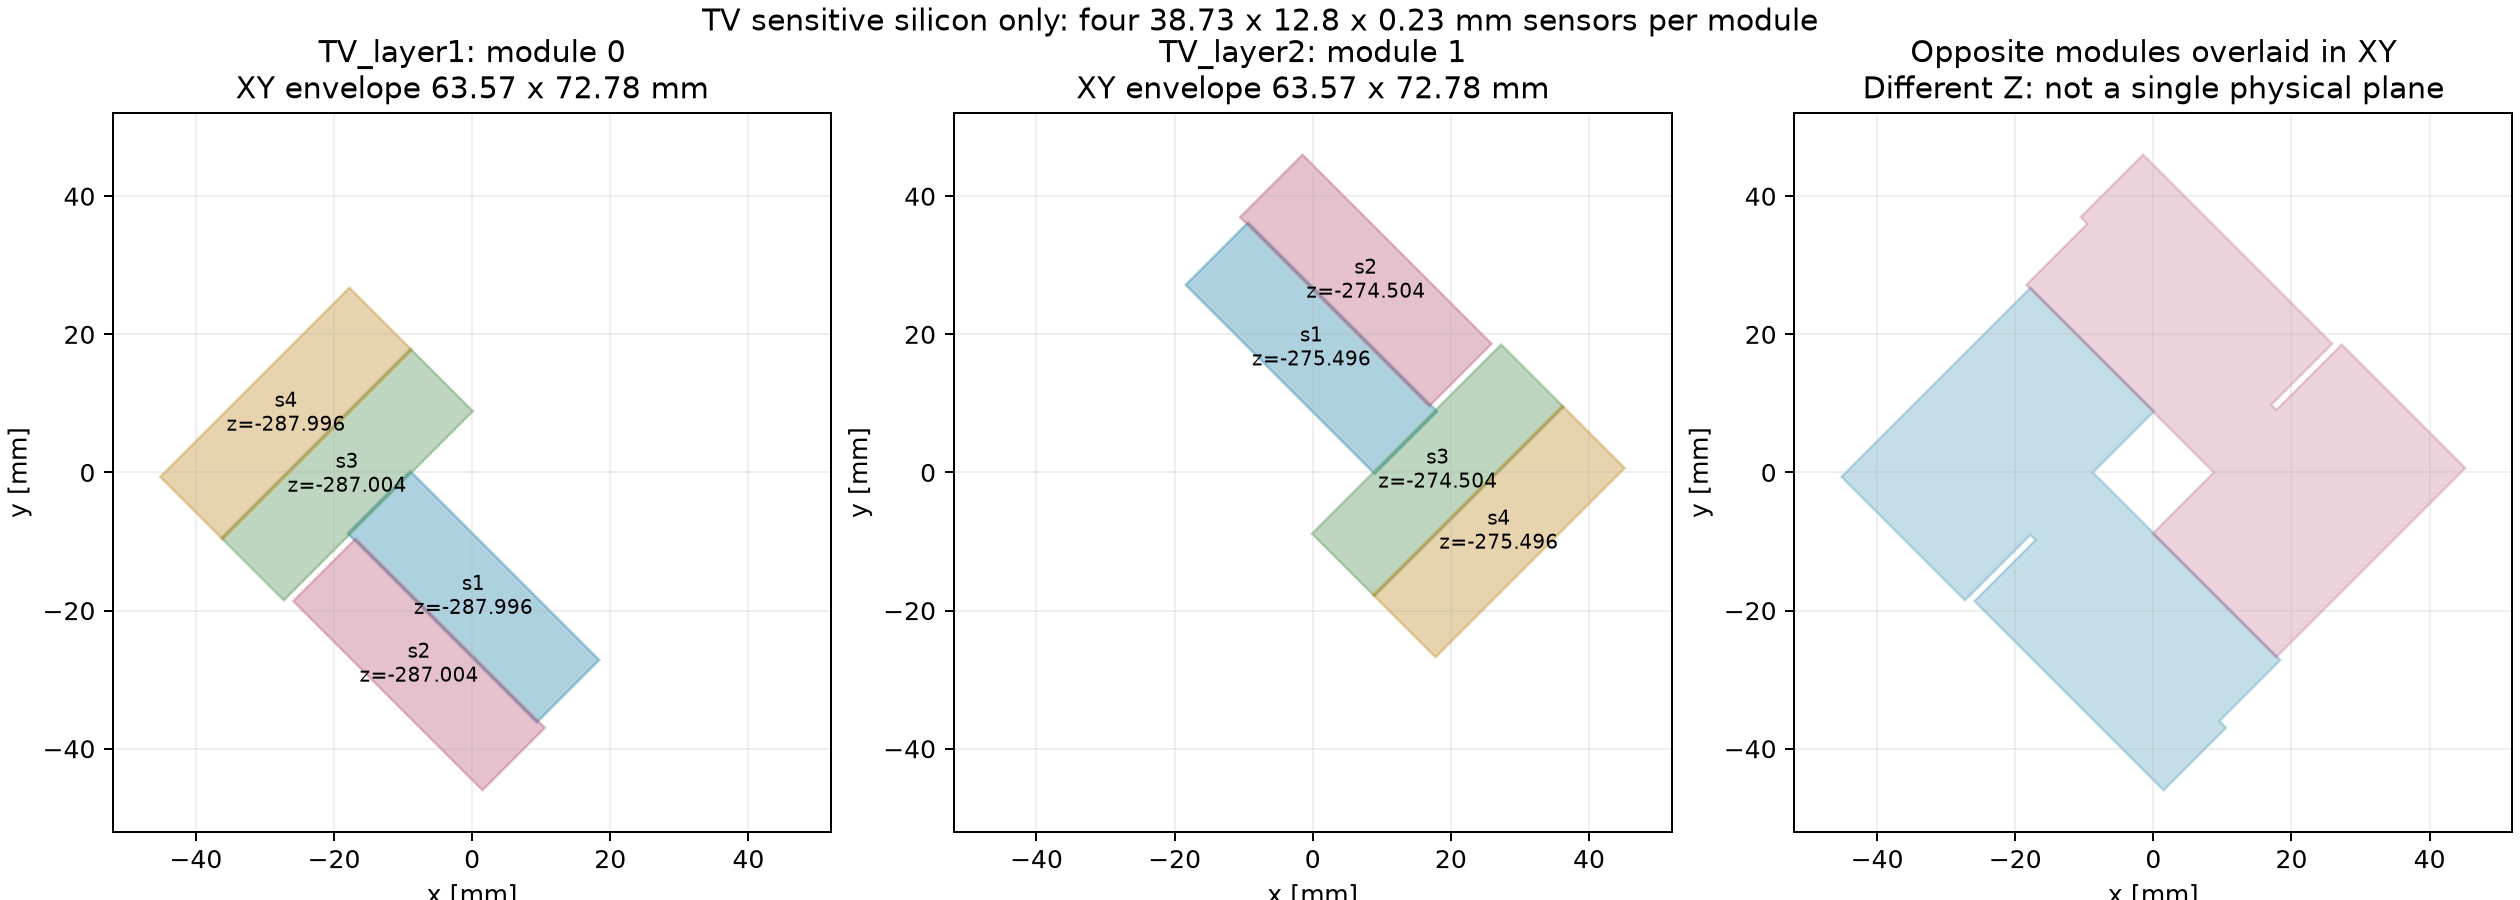
\includegraphics[width=\textwidth,height=.58\textheight,keepaspectratio]{../TV/review/tv_sensor_xy.png}\par
\small 200 sensitive-silicon sensors form 50 modules, represented by 100
sensor-centre planes. Left/right acceptances and sensor gaps are retained.\par
\vspace{2mm}
Sensor centres span $-287.996$ to 558.146 mm. From the origin, 29 modules are
downstream and 21 cannot fire. The earlier 20-plane square mockup is not used.
\end{frame}

\begin{frame}{TV and MT cuts returned by default}
\begin{tabularx}{\textwidth}{@{}lX@{}}
\toprule Property & Exact requirement \\
\midrule
\texttt{hasTV\_3Hits} & $n_{\rm TV}\geq3$ counted modules \\
\texttt{hasTV\_4Hits} & $n_{\rm TV}\geq4$ counted modules \\
\texttt{hasMT} & $(n_{\rm MP}\geq3)\lor(n_{\rm FT}\geq10)\lor
[(n_{\rm MP}\geq1)\land(n_{\rm FT}\geq6)]$ \\
\bottomrule
\end{tabularx}\par
\vspace{5mm}
MT thresholds are configurable using \texttt{MTSelection}, globally or
separately for each geometry. Changing a cut does not change the masks.\par
\vspace{3mm}
TV and UP are \textbf{not included} in \texttt{hasMT}. Apply the analysis's TV/UP
requirements separately. Keep the integer counts for later cut scans.
\end{frame}

\begin{frame}{How to read an output name}
\vspace{2mm}
\texttt{\color{teal}hasMT}\texttt{\_\color{blue}up\_y8x6\_ft\_8\_8\_10\_withHole}%
\texttt{\_\color{ink}magup}\par
\vspace{5mm}
\begin{tabularx}{\textwidth}{@{}lX@{}}
\toprule Part & Meaning \\
\midrule
\texttt{hasMT} & Property or count name \\
\texttt{up\_y8x6} & UP border choice \\
\texttt{ft\_8\_8\_10\_withHole} & FT widths and MP-derived hole \\
\texttt{magup} & Field-polarity prediction \\
\bottomrule
\end{tabularx}\par
\vspace{4mm}
\textbf{\PropertyCount{} properties $\times$ 6 geometries $\times$ 2 polarities
= \ColumnCount{} columns.}\par\vspace{2mm}
All arrays have one value per input track. Per-layer \texttt{fired\_*}
columns are omitted unless \texttt{include\_layer\_hits=True}.
\end{frame}

\begin{frame}{Counts and detector-presence flags}
\small
\begin{tabularx}{\textwidth}{@{}lllX@{}}
\toprule Count & Range & Presence flag & Interpretation \\
\midrule
\texttt{nTV} & 0--50 & \texttt{hasTV} & Fired modules; from the origin at most 29 reachable \\
\texttt{nUP} & 0--4 & \texttt{hasUP} & Four logical UP layers, not 16 independent counts \\
\texttt{nMP} & 0--5 & \texttt{hasMP} & Five simplified MP layers \\
\texttt{nFT} & 0--12 & \texttt{hasFT} & Four FT layers per station \\
\texttt{nRICH1} & 0--2 & \texttt{hasRICH1} & Radiator entry/exit acceptance planes \\
\texttt{nRICH2} & 0--2 & \texttt{hasRICH2} & Radiator entry/exit acceptance planes \\
\texttt{nPicoCal} & 0--2 & \texttt{hasPicoCal} & Simplified entry/exit surfaces \\
\texttt{nMUON} & 0--4 & \texttt{hasMUON} & Stations M2--M5 \\
\bottomrule
\end{tabularx}\par
\vspace{4mm}\normalsize Every presence flag means \textbf{count $>0$}, not full detector coverage.
Use \mbox{\texttt{nUP == 4}} or \mbox{\texttt{nFT == 12}} when all logical layers are required.
\end{frame}

\begin{frame}{RICH, PicoCal and Muon: useful canonical flags}
\small
\begin{tabularx}{\textwidth}{@{}lX@{}}
\toprule Flag & Meaning \\
\midrule
\texttt{hasRich1Entry}, \texttt{hasRich1Exit} & RICH1 plane hits \\
\texttt{hasRich2Entry}, \texttt{hasRich2Exit} & RICH2 plane hits \\
\texttt{hasRichEntry}, \texttt{hasRichExit} & OR of the corresponding RICH1/RICH2 hits \\
\texttt{hasPicoCal} & At least one PicoCal surface hit \\
\texttt{inPicoCal} & Both PicoCal entry and exit hit in the default layout \\
\texttt{nMuon}, \texttt{hasMuon} & Aliases for \texttt{nMUON}, \texttt{hasMUON} \\
\texttt{isMuon} & At least 3 Muon stations; adjustable with \texttt{min\_muon\_stations} \\
\bottomrule
\end{tabularx}\par
\vspace{4mm}\normalsize These are \textbf{geometric labels}: no Cherenkov PID, calorimeter response
or reconstructed muon identification is simulated.
\end{frame}

\begin{frame}{Additional volume flags and complete output reference}
For each of \texttt{RICH1}, \texttt{RICH2} and \texttt{PicoCal}, the API also returns:\par
\vspace{3mm}
\begin{tabularx}{\textwidth}{@{}lX@{}}
\toprule Property pattern & Meaning \\
\midrule
\texttt{<system>\_entry} & Entry plane fires \\
\texttt{<system>\_exit} & Exit plane fires \\
\texttt{<system>\_entry\_exit} & Entry AND exit fire \\
\texttt{<system>\_entry\_only} & Entry fires AND exit does not \\
\bottomrule
\end{tabularx}\par
\vspace{4mm}
The same geometry and polarity suffix is appended to \emph{every} property.\par
\vspace{3mm}
\texttt{tool\_output\_schema.json} lists all \ColumnCount{} exact column names,
their NumPy dtypes and values for two runnable example tracks.
\end{frame}

\begin{frame}[fragile]{Minimal runnable example}
\small
\begin{verbatim}
from xyshapes_detectors import PolarityComparison

states = dict(
    x=[0., 0.], y=[0., 0.], z=[0., 0.],
    tx=[.04, .02], ty=[.01, -.01],
    q_over_p=[1/20000., -1/50000.],
)
service = PolarityComparison.from_files(
    "MagField/magnetic_field_v5r0.root",
    map_polarity="magdown",
)
new_fields = service.label_tracks(states)
\end{verbatim}
\normalsize Positions are mm; $q/p$ is 1/MeV. Input slopes are $p_x/p_z$ and $p_y/p_z$.
Use each charged daughter's production point; $p_z>0$ is assumed.
\end{frame}

\begin{frame}{Example output: two tracks, one prediction}
\small \texttt{up\_y8x6\_ft\_8\_8\_10\_withHole\_magup}\par
\vspace{4mm}
\centering
\begin{tabular}{@{}lrrrrll@{}}
\toprule Track & nTV & nUP & nMP & nFT & hasMT & hasPicoCal \\
\midrule
\ExampleRows
\bottomrule
\end{tabular}\par
\vspace{5mm}
\normalsize Values are generated by running the preceding example against the
bundled field map, not hand-entered illustrations.\par
\vspace{3mm}
The same tracks also receive the other 11 geometry/polarity predictions.
The service does not filter, reorder or drop the input rows.
\end{frame}

\begin{frame}{Both polarities are predictions for the same tracks}
\begin{itemize}
\item The bundled map is labelled MagDown. The MagUp prediction reverses
\textbf{Bx, By and Bz together}; another map can declare its own reference polarity.
\item Each polarity requires a separate transport. Within that transport,
all six geometries reuse the same physical-plane crossings.
\item Keep both \texttt{\_magup} and \texttt{\_magdown} columns, then select the
appropriate ones using the data sample's actual magnet metadata.
\item Opposite-field flags do \textbf{not} measure the event's magnet polarity.
The two fields are ideal sign reversals, not separately measured maps.
\end{itemize}
\vspace{3mm}The same-sign comparisons isolate geometry changes; the same-geometry
comparisons isolate the field-polarity dependence.
\end{frame}

\begin{frame}[fragile]{Attach fields to daughters without losing decay alignment}
\small
\begin{verbatim}
output = dict(original_columns)
for daughter, states in daughter_state_columns.items():
    flags = service.label_tracks(states)
    output.update({f"{daughter}_{name}": values
                   for name, values in flags.items()})
\end{verbatim}
\normalsize
\begin{itemize}
\item Keep one row per candidate for fixed-daughter trees; prefix by daughter.
\item For jagged collections, restore track offsets after flattening.
\item Combine daughter flags into decay cuts in the analysis code.
\item Write a new output file or friend tree; ntuple I/O is not automatic.
\end{itemize}
\end{frame}

\begin{frame}{Scope and checks}
\begin{columns}[T,onlytextwidth]
\column{.47\textwidth}
\textbf{Included}\par\vspace{2mm}
Field-map interpolation, forward RK4 transport, XY acceptance at actual
surface $z$, logical-layer counts and configurable geometric cuts.\par\vspace{3mm}
\textbf{118 tests passed}: field/charge reversal, grouping, upstream masks,
MT thresholds, two-polarity consistency and track order.
\column{.47\textwidth}
\textbf{Not simulated}\par\vspace{2mm}
Material scattering, energy loss, sensor efficiencies, reconstruction,
detector response or PID.\par\vspace{3mm}
Failed/curling or incomplete transport raises \texttt{TrajectoryError}.
It must not be silently converted into an acceptance miss.
\end{columns}
\vspace{4mm}
Toy geometric acceptance is not a physics-sample efficiency. Use the sample's
track distribution, weights and denominator when comparing decay yields.
\end{frame}

\begin{frame}[fragile]{Start from a clone}
\small
\begin{verbatim}
git clone --branch feature/detector-mask-loader \
  https://github.com/qgl90/xyshapes_detetctors.git
cd xyshapes_detetctors
pip install -e '.[field]'
python -m unittest discover -s tests
\end{verbatim}
\normalsize The geometry masks and ROOT field map are included. ROOT itself
is not required for mask loading or propagation; uproot reads the field histograms.\par
\vspace{4mm}
\textbf{Usage:} \texttt{docs/decay\_study\_quickstart.md}\par
\textbf{API:} \texttt{docs/geometry\_comparison.md}\par
\textbf{Exact outputs:} \texttt{docs/geometry\_documentation/tool\_output\_schema.json}\par
\textbf{Geometry and TV studies:} \texttt{acceptance\_study\_summary.pdf}
\end{frame}
\end{document}
